\chapter{Knowledge representation}
\minitoc

\section{Introduction}

An AGI uses a KR structure to \textit{represent} the external world, and this structure is built with limited computational resources, and as such, must be approximate.  We have a lot of freedom to choose the KR format.

I chose logic as KR because it offers a \textit{direct} way to translate natural-language texts into machine knowledge.  This is of critical importance because the overall feasibility of AGI hinges on the efficiency of machine learning, and the most effective machine-learning method is ``learn by being told'' (\S\ref{sec:learn-by-being-told}).

A common misconception is:  ``How can complex ideas such as `John loves Mary' be reduced to logic formulae like \textit{loves(john,mary)}?''  One school of thought (see eg \citep*{Johnson-Laird1983}) posits that human reasoning is based on ``mental models'', but it is unclear how exactly they can be constructed.  My view of logic-based AI is that of using logic as a \textit{computational structure} for \textit{constructing} mental models.

% Sorted or unsorted logic?

\section{Multiplicity of knowledge representation schemes}

This is how I think of the issue of knowledge representation:\\
\begin{figure}[H]
\centering
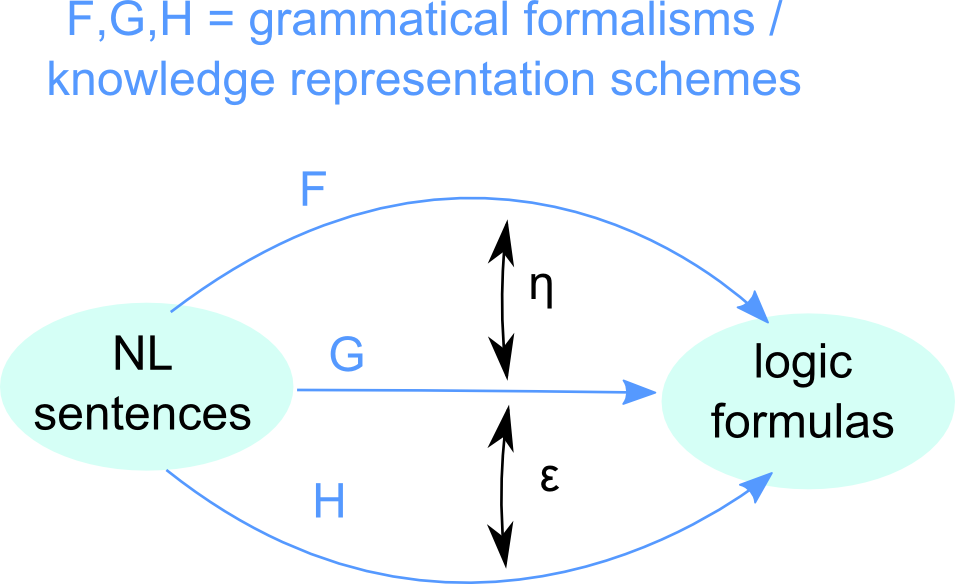
\includegraphics[scale=0.7]{KR-functors.png}
% \caption{KR functors}
\end{figure}

There are various KR schemes.  For example, in NL, there are various grammar formulations:\\
$F$ may be Phrase Structure Grammar\\
$G$ may be Fluid Construction Grammar\\
$H$ may be Categorial Grammar\\
$J$ may be Genifer's machine-learned grammar (which may be stochastic and inscrutable to humans)\\
$K$ may be some spatio-temporal KR scheme such as temporal logic, event calculus, situation calculus, etc

And then there would be transformations ($\eta, \epsilon, ...$) between the grammatical formalisms.

The problem is whether we can mix multiple KR schemes like $F$ and $G$.  The commonsense KB would be different under either $F$ or $G$, and the entire KB needs to be transformed by some $\eta$.

If we use $F, G, H,...$ at the same time, confusion may arise during machine learning and reasoning.

Perhaps, if we make Genifer be aware of transformations like $\eta, \epsilon, ...$ then maybe it can deal with multiple KR schemes at the same time?  Therefore we maybe don't need to choose or commit to any particular KR scheme at this stage...  in other words, any would be fine.

\section{Natural language}

Please also see the chapter on natural language (\ref{ch:natural-language}).

\subsection{Composition of concepts}
\label{sec:composition}

In 1928 the young Haskell Curry started working on \textbf{combinatory logic} (CL) as a \textit{logica universalis}, but it ran into inconsistency problems \footnote{In Genifer we try to use fuzzy-probabilistic truth values to get around this problem (see \S\ref{sec:paradox}).}.  One special feature of CL is \textbf{combinatorial completeness} -- meaning that any concept can, in principle, be applied to any other concept.  One can readily see that, when the concept of \textit{self-application} is applied to itself, it can lead to Russell's paradox (\S\ref{sec:paradox}).

Nevertheless, combinatorial completeness is something desirable in a universal logic.  It enables a logic to \textit{reason about logical paradoxes themselves}.  Bertrand Russell invented \textbf{type theory} to get around the problem of paradoxes, basically by banning all circular references.  But as a result of that, type theory (and thus the higher-order logic built on top of it) cannot be used to reason about paradoxes.

Curry's combinatory logic can represent arbitrary combinations of concepts, in a manner such as:\\
\tab $\lceil$wisdom$\rceil$ $\bullet$ $\lceil$socrates$\rceil$ = $\lceil$the wisdom of socrates$\rceil$

One of my latest insights is that the combination of concepts can be computed by the same process as \textbf{unification} of terms in logic.  For more details, refer to \S\ref{sec:unification}.

In 1963 JA Robinson discovered resolution, which is really unification + propositional refutation.  Unification decides if 2 terms can be made equationally identical.  Propositional refutation is an inference step that deals with the "calculus of thinking" at the \textit{sentence} level.

Around the 1900s, George Boole, CS Peirce, Gottlob Frege, amongst others, developed \textbf{predicate logic}, which is later popularized by people such Hilbert, Ackermann, Russell, and Whitehead.  Predacate logic has really been popular for only about 80 years, versus syllogistic logic that has been around since Aristotle's time.  Predicate logic differs from propositional logic by giving propositions \textit{internal structure} -- a proposition is broken down into a \textbf{predicate} and one or more \textbf{objects}.  However, this decomposition seems inadequate to deal with arbitrarily free combinations of concepts.

Combinatory logic provides a free way to compose terms via "application".  The key is to regard terms as (compound) concepts.  For example, in Genifer's notation:\\
\tab \english{tall handsome guy}\\
is the combination of the concepts\\
\tab (tall, handsome) $\circ$ guy.

Now, a few examples:\\
\english{tall handsome guy} is equivalent to \english{handsome tall guy};\\
\english{very tall guy} implies \english{tall guy};  but\\
\english{very tall guy} does not equal \english{tall very guy};

Thus the unification is modulo some special rules such as commutativity, associativity, etc, and certain reduction rules.  In other words, unification modulo a theory = "the calculus of concepts".

So we have a neat decomposition:\\
\tab calculus of thoughts = calculus of concepts + calculus of propositions

In \textbf{category theory}, one enforces the associative composition of arrows:\\
\tab $(ab)c = a(bc)$. \footnote{We often omit the application symbol $\circ$.}\\
Likewise, I observed that if we enforce the associative composition of concepts, the logical form becomes very elegant.  Due to associativity, any pair of concepts in an application:\\
\tab $a \circ b$\\
must be \textit{meaningful} in a meaningful sentence.

A consequence of enforcing associativity is that we can no longer use \textbf{Currying}.  For example:\\
\tab \english{John loves Mary}\\
would be rendered in Genifer's logic as\\
\tab \formula{((mary loves) john)}\\
rather than as suggested by Currying:\\
\tab \formula{((loves mary) john)}

Thus, in Genifer's logic, the 2 primitive operations are:\\
\tab 1. \textbf{application}, $\circ$\\
\tab 2. \textbf{pairing}, or cross product, $(a,b)$\\
with the associative and distributive rules:
$$ (a \circ b) \circ c = a \circ (b \circ c) $$
$$ (a, b) \circ c = (a \circ b, a \circ c)$$

One can recognize that this logic has the exactly form as a category.  \todo{I'm curious as to the role of exponentiation in this category?}

For more about how natural language sentences are translated into logical form, see the section on natural language and Geniform, \S\ref{sec:geniform}.

\subsubsection{Dynamic interpretation of semantics}

Look at these examples:\\
\tab \underline{glass slippers} are made of glass\\
\tab a \underline{door knob} is part of a door\\
\tab \underline{street prostitutes} work on the streets.\\
However,\\
\tab \underline{glass slippers} do not work in glasses\\
\tab a \underline{door knob} is not made of doors\\
\tab \underline{street prostitutes} are not part of the streets.

This suggests that the \textbf{semantics} of the compound concepts depend on \textit{external} pieces of knowledge, and hence must be interpreted \textit{dynamically}.  This is essentially the same idea as the abductive interpretation of natural language (\S\ref{sec:abduction-as-interpretation}).

\subsection{Reification}
\label{sec:reification}

Reification means ``to turn into objects''.  For example:\\
\tab \english{John loves Mary}\\
can be rendered as\\
\tab \formula{loves(john, mary)}\\
but\\
\tab \english{John loves Mary deeply}\\
would have to rendered as:\\
\tab \formula{love(love$_1$)} \tab \tab ; love$_1$ is an instance of love\\
\tab \formula{subject(love$_1$, john)}\\
\tab \formula{object(love$_1$, mary)}\\
\tab \formula{deep(love$_1$)}.

Notice that in the reified form, the original base-level formula:\\
\tab \formula{loves(john, mary)}\\
is lost!  This is rather unsatisfactory.

Geniform solves this problem by eliminating reification.

\section{Representing time}

As Einstein would have said, the representation scheme for space and time should be fundamentally the same.  As I have developed a vision theory (\S\ref{ch:vision}), I think temporal representations can follow a similar scheme.  OpenCog (http://www.opencog.org) is an AGI project more focused on embodiment, so we can also share their KR scheme.

\section{Contexts}

An excellent survey of contexts in logic-based AI is \citep*{Akman1996}.  The book \citep*{Sowa2000}, Chapter 5, is also excellent and contains additional insights about contexts.  Also the book \citep*{Bonzon2000}.

In Genifer, a context is just a set of propositions that are \textit{true in that context}.  This idea is very useful in the clustering of the KB for inference speed-up (\S\ref{sec:hi-oracle}).

\section{Assumptions and counterfactuals}

How to make assumptions during inference?  \english{Assuming mom is at home, I call her phone number.}

Example of a counterfactual conditional:  \english{If Oswald did not kill kennedy, someone else would have.}
